\cleardoublepage\chapter{Introduction}
\minitoc\label{sec:introduction}\vspace{.5cm}

\section{Background and Motivation}
A physical tunnel allows vehicles to move between 2 places indepently from surrounding geography. 
Similarly, network tunneling is a mean to organize traffic between host A and B in a way that:

\begin{itemize}
    \item Abstracts the underlying path over the public network: Applications binding to the tunnel are not aware of the real paths that packets take.
    \item Encapsulates and encrypts: Middle man - even can intercept the traffic - can't always determine if a network frame belongs to the tunnel or a tunnel is being used, nor decrypt the content.
\end{itemize}

A \ac{VPN} is a application build on top of a tunnel to connect 2 networks, effectively allow its host to access the other internal network remotely.
Well known \ac{VPN} applications can be named: \ac{wgpage}, \ac{ovpnpage}, IPsec, PPTP, PPPoE, L2TP, ...
Although different in level of operation (Network layer, Data Link layer) and operation space (kernel or user space), they generally share the same concept of single link: the tunnel utilizes one single network link to transmit and receive the tunnel packets. 
The other concept, namely \textit{multipath}, would deploy multiple network links so it can achieve higher reliability through redundancy or higher bandwidth through combining links, even though these characteristics are more relevant to environment such as infrastructure, datacenter or industrial application rather than end-user usage.
There are protocols such as \ac{MPTCP}, \ac{SCTP} that implement the concept, albeit in form of non-sharable connection.
A non-share connection is initiated similarly to initiating a socket and can only be used by by the caller program. 
This severly limits the capability to control, schedule and share multipath resources between multiple applications in an effective manner, i.e prioritizing, buffering ... 
These require centralized orchestration level of control over all communication channels by a control plane, which doesn't exist for these protocols.

We propose another tunnel implementation: \ac{MTX}. 
The tunnel will have multipath support by design, allow multiple applications to share the connection simultainously, and be built based on Linux's \ac{xdppage} socket family.
Using the latest native Linux's technology, the implementation is expected to performance-wise outperform any userspace implementation while retain compatibility with existing systems and code base's simplicity. 
Support for multiple connection links offers reliability, large raw-bandwidth and a rich set of configuration to appications binding to the tunnel, makes it suitable for high demand use-cases such as industry, data center, telecommunication hub. 
In this document, an enhancement for the 5G's GTP-U protocol with \ac{MTX} library will be investigated. GTP-U is the protocol that helps UPF and gNodeB functions of a 5G system communicating, which demands both bandwidth and stability and therefore is a suitable match for a \ac{MTX} demostration.


\section{Problem Statement}\index{Requirements}

% \sidenote{State of the Art}
% \todomid{write about the State of the Art}

% \sidenote{Issue:\\Example 1}
% \todomid{write about the first issue}

% \sidenote{Issue:\\Example 2}
% \todomid{write about the second issue}

% \sidenote{Synopsis}
% \todomid{write about the synopsis of the issues and \Cref{fig:intro:c}}

% \begin{figure}[htbp]
%     \centering
%     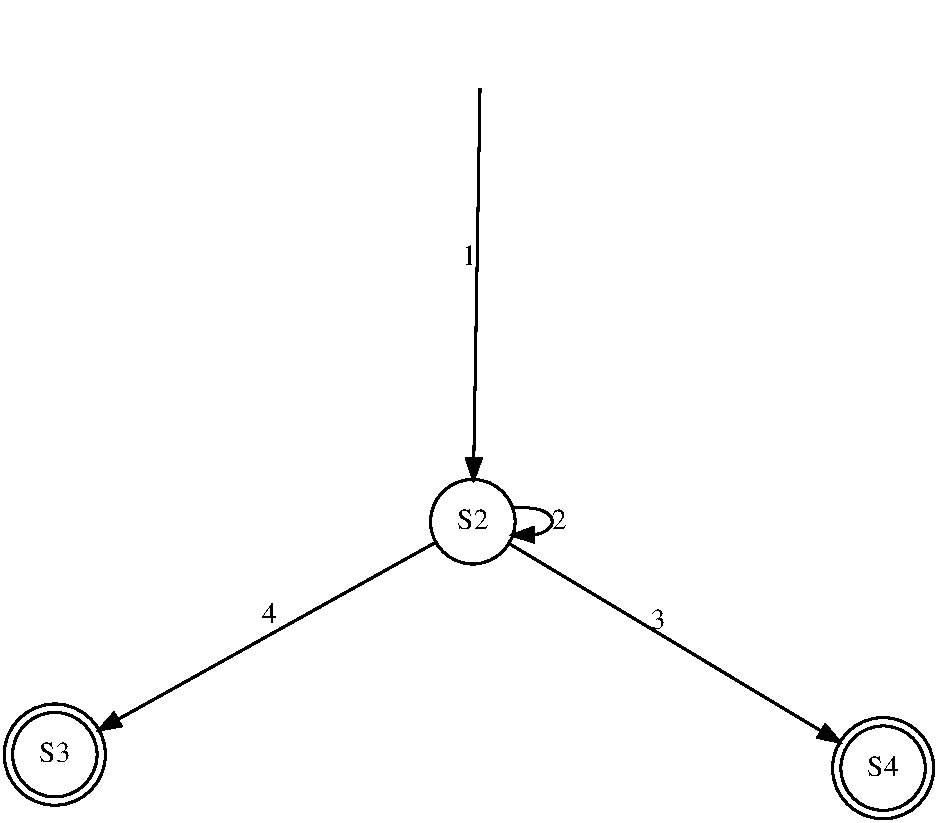
\includegraphics[width=.5\textwidth]{resources/images/job_lifecycle}
%     \caption{Relationship between issues}\label{fig:intro:c}
% \end{figure}

\section{Assumptions and Scope}

% \sidenote{Research Assumptions}
% \todomid{write about the research assumptions~\cite{li2002design}}

% \sidenote{Research Scope}
% \todomid{write about the research scope --- \Cref{fig:intro:a,fig:intro:b,fig:intro:c}}


\section{Objectives and Contributions}

% \begin{figure}[htbp]
%     \centering
%     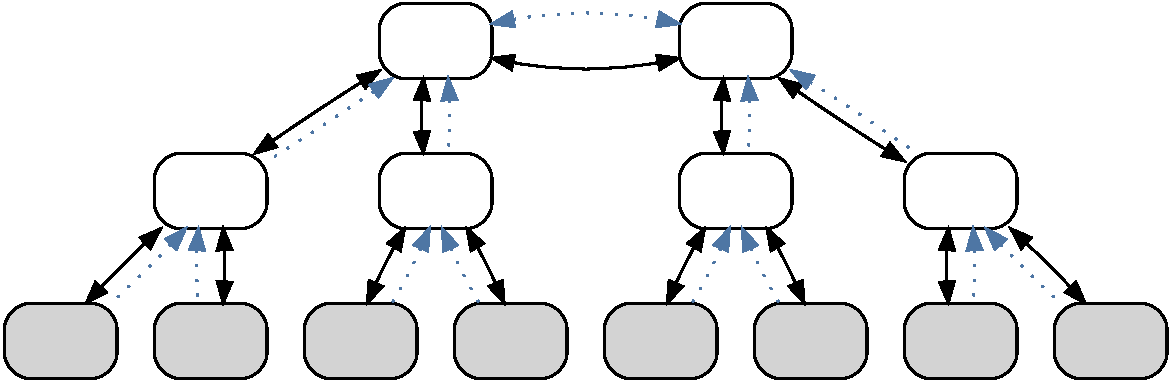
\includegraphics[width=.55\textwidth]{resources/images/example3}
%     \caption{Structure of research}\label{fig:intro:struct}
% \end{figure}

% \sidenote{Research Objectives \& Contributions}
% \todomid{write about the research objectives and \ac{DBpedia} and \Cref{fig:intro:struct}}

% \section{Methodology and Outline}

% \todomid{write about the research outline and \Cref{fig:intro:methodology}. Summarize \Cref{sec:introduction,sec:sota,sec:reqs,sec:contrib1,sec:contrib2,sec:contrib3,sec:eval,sec:summary}.}

% \begin{sidewaysfigure}
%     \centering
%     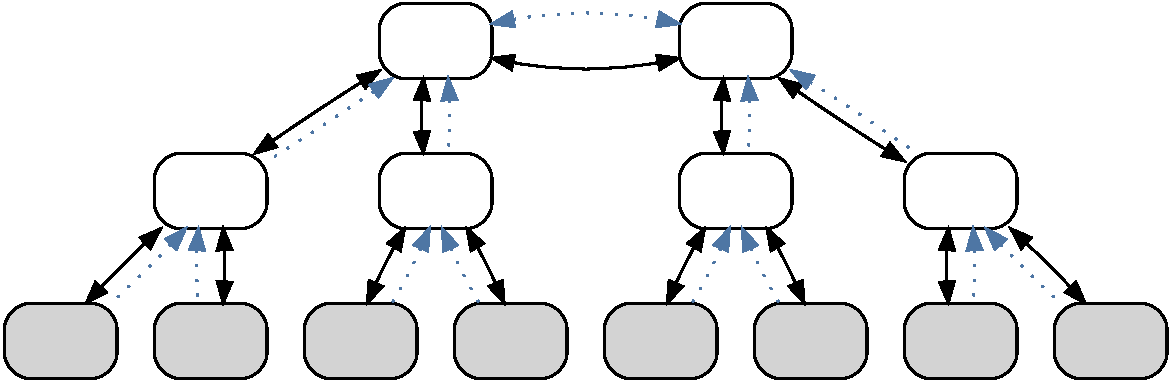
\includegraphics[width=.7\textwidth]{resources/images/example3}
%     \caption{Workflow of the research and structure of the thesis}\label{fig:intro:methodology}
% \end{sidewaysfigure}
